%% LaTeX Document
%% Author: Jose Pablo Apú, Jose Carlos Campos, Jorge Soto
%% Document Class
\documentclass[11pt]{article}
%%*************************************************************************
%% Most used packages
\usepackage{graphicx}				%%include figures
\usepackage[utf8]{inputenc}			%%include latin characters
\usepackage[english]{babel}			%%spanish
\usepackage[vmargin=4cm,			%%margins
	    tmargin=3cm,
	    hmargin=2cm,
	    letterpaper]{geometry}
\usepackage{color}				%%include colors
\usepackage{fancyhdr}				%%use fancy headers and footes
%\usepackage{framed}				%%framed boxes
\usepackage{hyperref}				%%make hyperlinks
%%*************************************************************************
%% Other settings
\definecolor{shadecolor}{rgb}{1,0.8,0.3}	%%boxes color
\setlength{\parindent}{0pt}			%%indemptation
\pagestyle{fancy}				%%needed to include fancy styles
\renewcommand{\headrulewidth}{0.25mm}		%%linewidth of the headers
\pagenumbering{gobble}				%%remove the page number
\graphicspath{{../multimedia/imagenes/}}	%%multimedia path
%%*************************************************************************
%% Fancy Header
%% EIE's template
\fancyhead[L]{
\includegraphics[scale=0.15]{ucr}}
\fancyhead[C]{UNIVERSIDAD DE COSTA RICA\\
	      ESCUELA DE INGENIERÍA ELECTRICA\\
	      ESTRUCTURAS ABSTRACTAS DE DATOS Y ALGORITMOS\\
	      PARA INGENIERIA - IE0217\\
	      PROYECTO I - PROPUESTA}
\fancyhead[R]{
\includegraphics[scale=0.4]{eie}}
\pagestyle{fancy}
\setlength{\headheight}{60pt}
%%*************************************************************************
\begin{document}

\begin{center}
{ \huge \bfseries Data Computing Visualization Library }\\[0.2cm]
{ Jose Carlos Campos - Jose Pablo Apu - Jorge Soto }\\[0.2cm]
\rule{\linewidth}{0.25mm}
\end{center}

\subsection*{Introducción}
Con el fin de brindar una mayor facilidad para visualizar los datos, 
la idea es crear una libreria, en c++, que tome los datos a traves de una 
base de datos y los despliegue en pantalla de una manera grafica. Para lograr 
dicha tarea se utilizara mysql como manejador de bases de datos, utilizando 
la libreria mysql++ y para visualizar los datos de manera grafica se piensa 
utilizar la libreria llamada plot++. Además se pretende implementar un set 
de herramientas para obtener datos estadísticos de los datos obtenidos de la base de datos. 

\subsection*{Justificación}
La librería será diseñada para que cualquier usuario de MySql pueda utilizarla.
La visualización de datos permite un mejor análisis y una mayor comprensión 
de los mismos. En una base de datos, la información es prácticamente números 
y letras únicamente. Al graficar dicha información, se puede entender de una mejor
manera el significado de los datos.

Cuando se tiene una gran cantidad de información, millones de datos individuales, 
es dificil poder interpretar la información y analizarla para así poder tomar
una decisión con base en los resultados obtenidos. Para poder darle un sentido
de forma eficiente a esta gran cantidad de información se tiene por respuesta 
la visualización de datos. Pero también se debe seleccionar la visualización
apropiada para un conjunto de datos determinado, ya que no todos los métodos 
de graficación son apropiados para describir los resultados obtenidos.\cite{oreilly} 

En el nivel emprasarial, se debe hacer uso de herramientas de visualización de datos.
La cantidad de datos es proporcional al tamaño de la empresa. Teniendo muchos datos, 
es más dificil encontrar patrones y relaciones para la correcta toma de decisiones. 
Se necesita elegir de manera rápida y precisa las decisiones de negocios para que 
la empresa permanezca competitiva.\cite{dundas}

\subsubsection*{Objetivo General}
Diseñar una biblioteca que permita la visualización de la información en una base de datos.

\subsubsection*{Objetivos Específicos}
\begin{itemize}
\item Implementar un módulo que utilice mysql++ para que importe una serie de datos desde MySql 
      y los convierta en información compatible para la librería que grafica.
\item Implementar un conjunto de herramientas matemáticas que permitan un análisis
	  estadístico cuantitativo de los datos.
\item Implementar un modulo que permita el análisis cualitativo de la información mediante 
	  distintas técnicas de visualización de datos.
\end{itemize}

\subsection*{Metodología}
Mediante la utilización de librerías ya creadas, como lo son mysql++, sfml 
y gnuplot o bien openGL, se creará herramientas para facilitar al programador 
visualizar un conjunto de datos. Para esto se utilizará principalmente el
lenguaje de programación C++ y el paradigma de programación orientada a objetos.

\begin{table}[ht]
\caption{Métodos que se esperan implementar} % title of Table
\centering % used for centering table
\begin{tabular}{p{4cm} p{12cm}} % centered columns (4 columns)
\hline\hline %inserts double horizontal lines
\\
Método & Descripción \\ [0.5ex] % inserts table 
%heading
\hline % inserts single horizontal line
\\

Conexión a MySQL & Se espera que los datos provengan de una base de datos, por lo que es necesario vincular estos datos con el módulo que grafica. \\ % inserting body of the table

\\

Query de MySQL & Para interpretar los datos, es necesario acomodar, o bien optener información importante para generar la gráfica. Para se utiliza el motor de MySQL para aprovechar dicha facilidad \\

\\

Obtener la media, la desviación estandar, y la varianza & de esto se encarga MySQL y funciona para obtener las gráficas de media y la distribucuión gaussiana. \\

\\

Kde y Jitterplor & Son funciones que sirven para... y que pueden ser generadas mediante gnuplot. \\
\hline %inserts single line
\end{tabular}
\label{table:nonlin} % is used to refer this table in the text
\end{table}

\subsection*{Cronograma}

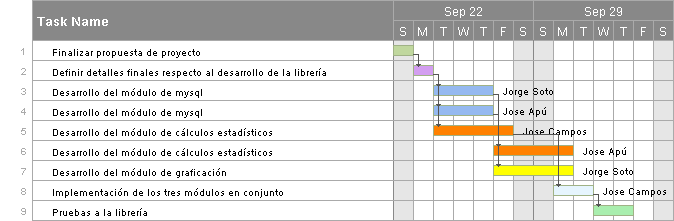
\includegraphics[scale=0.7]{ganttChart}

%% References
\begin{thebibliography}{10}
\bibitem{tangent}\url{http://tangentsoft.net/mysql++/}
\bibitem{opengl}\url{http://www.opengl.org/}
\bibitem{sfml}\url{http://www.sfml-dev.org/}
\bibitem{oreilly}Steele, J., \textit{Why data visualization matters}, 
		\url{http://strata.oreilly.com/2012/02/why-data-visualization-matters.html}
\bibitem{dundas}Dundas Data Visualization, Inc., \textit{Making Business Decisions Easier with Data Visualizations}
		\url{http://www.dundas.com/discover/article/making-business-decisions-easier-with-data-visualizations/}
\end{thebibliography}
%%*************************************************************************	
\end{document}
